% Options for packages loaded elsewhere
% Options for packages loaded elsewhere
\PassOptionsToPackage{unicode}{hyperref}
\PassOptionsToPackage{hyphens}{url}
\PassOptionsToPackage{dvipsnames,svgnames,x11names}{xcolor}
%
\documentclass[
  9.5pt,
]{article}
\usepackage{xcolor}
\usepackage[top=12mm,bottom=12mm,left=12mm,right=12mm]{geometry}
\usepackage{amsmath,amssymb}
\setcounter{secnumdepth}{5}
\usepackage{iftex}
\ifPDFTeX
  \usepackage[T1]{fontenc}
  \usepackage[utf8]{inputenc}
  \usepackage{textcomp} % provide euro and other symbols
\else % if luatex or xetex
  \usepackage{unicode-math} % this also loads fontspec
  \defaultfontfeatures{Scale=MatchLowercase}
  \defaultfontfeatures[\rmfamily]{Ligatures=TeX,Scale=1}
\fi
\usepackage{lmodern}
\ifPDFTeX\else
  % xetex/luatex font selection
\fi
% Use upquote if available, for straight quotes in verbatim environments
\IfFileExists{upquote.sty}{\usepackage{upquote}}{}
\IfFileExists{microtype.sty}{% use microtype if available
  \usepackage[]{microtype}
  \UseMicrotypeSet[protrusion]{basicmath} % disable protrusion for tt fonts
}{}
\makeatletter
\@ifundefined{KOMAClassName}{% if non-KOMA class
  \IfFileExists{parskip.sty}{%
    \usepackage{parskip}
  }{% else
    \setlength{\parindent}{0pt}
    \setlength{\parskip}{6pt plus 2pt minus 1pt}}
}{% if KOMA class
  \KOMAoptions{parskip=half}}
\makeatother
% Make \paragraph and \subparagraph free-standing
\makeatletter
\ifx\paragraph\undefined\else
  \let\oldparagraph\paragraph
  \renewcommand{\paragraph}{
    \@ifstar
      \xxxParagraphStar
      \xxxParagraphNoStar
  }
  \newcommand{\xxxParagraphStar}[1]{\oldparagraph*{#1}\mbox{}}
  \newcommand{\xxxParagraphNoStar}[1]{\oldparagraph{#1}\mbox{}}
\fi
\ifx\subparagraph\undefined\else
  \let\oldsubparagraph\subparagraph
  \renewcommand{\subparagraph}{
    \@ifstar
      \xxxSubParagraphStar
      \xxxSubParagraphNoStar
  }
  \newcommand{\xxxSubParagraphStar}[1]{\oldsubparagraph*{#1}\mbox{}}
  \newcommand{\xxxSubParagraphNoStar}[1]{\oldsubparagraph{#1}\mbox{}}
\fi
\makeatother


\usepackage{longtable,booktabs,array}
\newcounter{none} % for unnumbered tables
\usepackage{calc} % for calculating minipage widths
% Correct order of tables after \paragraph or \subparagraph
\usepackage{etoolbox}
\makeatletter
\patchcmd\longtable{\par}{\if@noskipsec\mbox{}\fi\par}{}{}
\makeatother
% Allow footnotes in longtable head/foot
\IfFileExists{footnotehyper.sty}{\usepackage{footnotehyper}}{\usepackage{footnote}}
\makesavenoteenv{longtable}
\usepackage{graphicx}
\makeatletter
\newsavebox\pandoc@box
\newcommand*\pandocbounded[1]{% scales image to fit in text height/width
  \sbox\pandoc@box{#1}%
  \Gscale@div\@tempa{\textheight}{\dimexpr\ht\pandoc@box+\dp\pandoc@box\relax}%
  \Gscale@div\@tempb{\linewidth}{\wd\pandoc@box}%
  \ifdim\@tempb\p@<\@tempa\p@\let\@tempa\@tempb\fi% select the smaller of both
  \ifdim\@tempa\p@<\p@\scalebox{\@tempa}{\usebox\pandoc@box}%
  \else\usebox{\pandoc@box}%
  \fi%
}
% Set default figure placement to htbp
\def\fps@figure{htbp}
\makeatother


% definitions for citeproc citations
\NewDocumentCommand\citeproctext{}{}
\NewDocumentCommand\citeproc{mm}{%
  \begingroup\def\citeproctext{#2}\cite{#1}\endgroup}
\makeatletter
 % allow citations to break across lines
 \let\@cite@ofmt\@firstofone
 % avoid brackets around text for \cite:
 \def\@biblabel#1{}
 \def\@cite#1#2{{#1\if@tempswa , #2\fi}}
\makeatother
\newlength{\cslhangindent}
\setlength{\cslhangindent}{1.5em}
\newlength{\csllabelwidth}
\setlength{\csllabelwidth}{3em}
\newenvironment{CSLReferences}[2] % #1 hanging-indent, #2 entry-spacing
 {\begin{list}{}{%
  \setlength{\itemindent}{0pt}
  \setlength{\leftmargin}{0pt}
  \setlength{\parsep}{0pt}
  % turn on hanging indent if param 1 is 1
  \ifodd #1
   \setlength{\leftmargin}{\cslhangindent}
   \setlength{\itemindent}{-1\cslhangindent}
  \fi
  % set entry spacing
  \setlength{\itemsep}{#2\baselineskip}}}
 {\end{list}}
\usepackage{calc}
\newcommand{\CSLBlock}[1]{\hfill\break\parbox[t]{\linewidth}{\strut\ignorespaces#1\strut}}
\newcommand{\CSLLeftMargin}[1]{\parbox[t]{\csllabelwidth}{\strut#1\strut}}
\newcommand{\CSLRightInline}[1]{\parbox[t]{\linewidth - \csllabelwidth}{\strut#1\strut}}
\newcommand{\CSLIndent}[1]{\hspace{\cslhangindent}#1}



\setlength{\emergencystretch}{3em} % prevent overfull lines

\providecommand{\tightlist}{%
  \setlength{\itemsep}{0pt}\setlength{\parskip}{0pt}}



 


\usepackage{booktabs}
\usepackage{array}
\usepackage{microtype}
\setlength{\parskip}{3pt}
\setlength{\parindent}{0pt}
\setlength{\tabcolsep}{4pt}
\makeatletter
\@ifpackageloaded{tcolorbox}{}{\usepackage[skins,breakable]{tcolorbox}}
\@ifpackageloaded{fontawesome5}{}{\usepackage{fontawesome5}}
\definecolor{quarto-callout-color}{HTML}{909090}
\definecolor{quarto-callout-note-color}{HTML}{0758E5}
\definecolor{quarto-callout-important-color}{HTML}{CC1914}
\definecolor{quarto-callout-warning-color}{HTML}{EB9113}
\definecolor{quarto-callout-tip-color}{HTML}{00A047}
\definecolor{quarto-callout-caution-color}{HTML}{FC5300}
\definecolor{quarto-callout-color-frame}{HTML}{acacac}
\definecolor{quarto-callout-note-color-frame}{HTML}{4582ec}
\definecolor{quarto-callout-important-color-frame}{HTML}{d9534f}
\definecolor{quarto-callout-warning-color-frame}{HTML}{f0ad4e}
\definecolor{quarto-callout-tip-color-frame}{HTML}{02b875}
\definecolor{quarto-callout-caution-color-frame}{HTML}{fd7e14}
\makeatother
\makeatletter
\@ifpackageloaded{caption}{}{\usepackage{caption}}
\AtBeginDocument{%
\ifdefined\contentsname
  \renewcommand*\contentsname{Table of contents}
\else
  \newcommand\contentsname{Table of contents}
\fi
\ifdefined\listfigurename
  \renewcommand*\listfigurename{List of Figures}
\else
  \newcommand\listfigurename{List of Figures}
\fi
\ifdefined\listtablename
  \renewcommand*\listtablename{List of Tables}
\else
  \newcommand\listtablename{List of Tables}
\fi
\ifdefined\figurename
  \renewcommand*\figurename{Figure}
\else
  \newcommand\figurename{Figure}
\fi
\ifdefined\tablename
  \renewcommand*\tablename{Table}
\else
  \newcommand\tablename{Table}
\fi
}
\@ifpackageloaded{float}{}{\usepackage{float}}
\floatstyle{ruled}
\@ifundefined{c@chapter}{\newfloat{codelisting}{h}{lop}}{\newfloat{codelisting}{h}{lop}[chapter]}
\floatname{codelisting}{Listing}
\newcommand*\listoflistings{\listof{codelisting}{List of Listings}}
\makeatother
\makeatletter
\makeatother
\makeatletter
\@ifpackageloaded{caption}{}{\usepackage{caption}}
\@ifpackageloaded{subcaption}{}{\usepackage{subcaption}}
\makeatother
\usepackage{bookmark}
\IfFileExists{xurl.sty}{\usepackage{xurl}}{} % add URL line breaks if available
\urlstyle{same}
\hypersetup{
  pdftitle={Predicting car safety-feature bundle choices},
  pdfauthor={Imelda Lee; Woon Zee Ning; Clarence Elvareta; Sng Zhenhao},
  colorlinks=true,
  linkcolor={blue},
  filecolor={Maroon},
  citecolor={Blue},
  urlcolor={Blue},
  pdfcreator={LaTeX via pandoc}}


\title{Predicting car safety-feature bundle choices}
\usepackage{etoolbox}
\makeatletter
\providecommand{\subtitle}[1]{% add subtitle to \maketitle
  \apptocmd{\@title}{\par {\large #1 \par}}{}{}
}
\makeatother
\subtitle{Discrete-choice structure, observed heterogeneity, and robust
validation}
\author{Imelda Lee \and Woon Zee Ning \and Clarence Elvareta \and Sng
Zhenhao}
\date{}
\begin{document}
\maketitle


\begin{tcolorbox}[enhanced jigsaw, arc=.35mm, bottomrule=.15mm, bottomtitle=1mm, breakable, colback=white, colbacktitle=quarto-callout-note-color!10!white, colframe=quarto-callout-note-color-frame, coltitle=black, left=2mm, leftrule=.75mm, opacityback=0, opacitybacktitle=0.6, rightrule=.15mm, title=\textcolor{quarto-callout-note-color}{\faInfo}\hspace{0.5em}{Note}, titlerule=0mm, toprule=.15mm, toptitle=1mm]

This report was generated with AI assistance under human direction. The
analysis, model selection, and numerical results were produced and
checked by the project team, and the final text has been reviewed and
checked by the project team before submission.

\end{tcolorbox}

\section{Problem, data, and
validation}\label{problem-data-and-validation}

The task is to predict which of four car safety-feature bundles a
respondent chooses. Alternatives 1--3 contain 19 safety-attribute level
codes and a price; alternative 4 is a designed no-purchase option with
every attribute and price fixed at zero. The training data contain
21,565 choice tasks from 1,135 respondents, each completing exactly 19
tasks. The test data contain 4,997 tasks from 263 entirely new
respondents. The outcome is evaluated by four-class log loss,

\[
\mathrm{LogLoss}=-\frac{1}{N}\sum_{i=1}^{N}\sum_{j=1}^{4}
y_{ij}\log(p_{ij}),
\]

for which uniform probabilities score 1.38629. The no-purchase option is
chosen 30.2\% of the time, rising from about 24\% at Task 1 to 34\% at
Tasks 15--19. Consequently, both the inside-bundle comparison and survey
fatigue matter.

The separation of respondents is the central validation constraint.
Cases 1--1,135 occur only in train and Cases 1,136--1,398 only in test;
therefore, random effects or memorized respondent preferences cannot
transfer. A row-level split would also leak up to 18 tasks from the same
person into the validation training set. We instead used an 80/20
respondent holdout (seed 7402) for rapid screening and
respondent-grouped five-fold cross-validation (seed 4821) for
confirmation. All reported cross-validation (CV) scores pool the
out-of-fold predictions before calculating log loss. Model improvements
were judged by paired respondent bootstrap comparisons, whose standard
deviation was about 0.001, rather than by coefficient significance
alone.

\section{Best model: ensemble\_v11 + neural ensemble diversity +
set-context network + segment-shift
pruning}\label{best-model-ensemble_v11-neural-ensemble-diversity-set-context-network-segment-shift-pruning}

Our best submitted model adds a set-context feed-forward network on top
of the earlier \textbf{ensemble\_v11 + MLP}, then prunes two
structurally unreliable terms from its logit component:

\[
\hat{\mathbf p}=0.889\,\hat{\mathbf p}_{\text{v11+mlp}}+0.111\,\hat{\mathbf p}_{\text{setctx}},
\qquad
\hat{\mathbf p}_{\text{v11+mlp}}=0.85\,\hat{\mathbf p}_{\text{v11}}+0.15\,\hat{\mathbf p}_{\text{mlp}},
\qquad
\hat{\mathbf p}_{\text{v11}}=0.80\,\hat{\mathbf p}_{\text{m8trpg}}+
0.20\,\hat{\mathbf p}_{\text{xgb}}.
\]

The set-context addition achieves \textbf{1.143533 respondent-grouped CV
log loss and 1.200 public leaderboard log loss}, improving on both
counts over ensemble\_v11+MLP (1.143789 CV / 1.201 public) and
substantially over the 1.38629 benchmark. Its canonical-split confidence
interval was a wide near-miss, but six additional independent fold-seed
assignments (repeated cross-validation) strengthened the signal rather
than weakening it--the reverse of this project's usual near-miss
pattern--and cleared our pre-stated significance bar. This is the second
refinement, out of many dozens tested after ensemble\_v11, whose
public-leaderboard result was checked against its CV-predicted direction
and matched (Section 3.3).

A final refinement, \textbf{segment-shift pruning}, then improved
\texttt{m8trpg} itself. A structural audit (Section 3) found that two of
its already-deployed market-segment terms (\texttt{In\_seg3},
\texttt{In\_seg5}, capturing segments 3 and 5's opt-out-margin
deviation) are statistically indistinguishable from zero on the full
training set (p=0.758, p=0.404) even though their
\emph{price-sensitivity} counterparts are highly significant
(p\textless1e-10)--and segments 3 and 5 are exactly the segments whose
share of the loss function explodes from 9.4\% in training to 68.8\% in
test. Dropping only these two terms improved respondent-grouped CV,
propagated through the full ensemble, from \textbf{1.143533 to 1.143255}
(repeated CV: 6/6 seeds positive, 95\% CI {[}0.0000441, 0.0003292{]},
excluding zero). This is our final selected Kaggle submission:
\textbf{1.200 public, 1.199 private} leaderboard log loss, now that the
competition has closed and the private score is visible (Section 3).

\subsection{Structured conditional-logit
component}\label{structured-conditional-logit-component}

The main component, \textbf{m8trpg}, is a conditional logit estimated
with \texttt{mlogit} (Croissant 2020). Alternative 4 has utility fixed
at zero. For each inside alternative, utility contains:

\begin{itemize}
\item
  dummy-coded levels for all 19 safety attributes, avoiding an
  unjustified linear-in-code assumption;
\item
  a saturated main effect for price levels 2--12;
\item
  indicators for being cheapest or dearest within the three-bundle
  choice set, plus distances from the cheapest and dearest prices;
\item
  alternative dummies for positions 2 and 3;
\item
  linear price and inside-good interactions with observed respondent
  heterogeneity: income, age, mileage, night driving, market segment,
  task position, region, and parking availability, with selected
  inside-good interactions for gender, urbanicity, and education.

  \begin{center}
  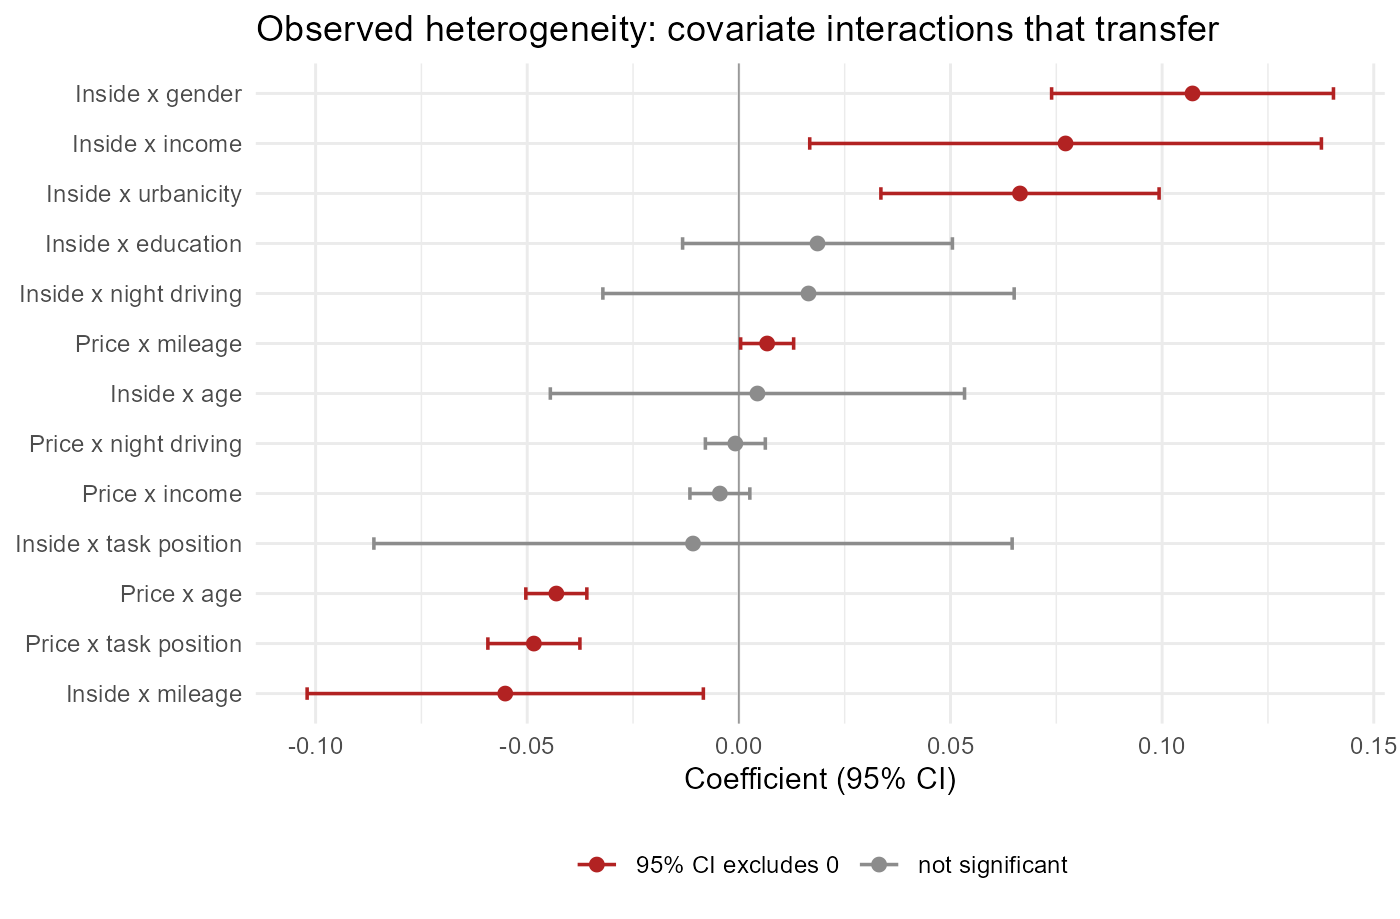
\includegraphics[width=0.6\linewidth,height=\textheight,keepaspectratio]{tae1.png}
  \end{center}
\end{itemize}

Respondent covariates cannot enter conditional logit as uninteracted
main effects because they are constant across the four alternatives and
cancel from the choice probability. Interacting them with price or an
inside-good indicator lets observed heterogeneity transfer to unseen
respondents. Task-position terms capture the increasing no-purchase rate
across the 19-task survey. On its own, m8trpg scores \textbf{1.147021
CV}.

\subsubsection{Price identification and choice-set
context}\label{price-identification-and-choice-set-context}

Price produced the most important late-stage modeling advance. Earlier
models treated it as one continuous slope even though every safety
attribute was dummy-coded. A full price factor initially caused an
exactly singular Hessian. This was not a numerical optimizer failure:
design-matrix QR diagnostics exposed a structural rank-one dependency.
Every inside bundle has exactly 9 of its 19 attributes at a
non-reference level, so

\[
\frac{1}{9}\sum_{k=1}^{19} I(\text{attribute }k\ne 0)
=I(\text{inside bundle})
=\sum_{\ell=1}^{12} I(\text{Price}=\ell).
\]

Thus, the attribute block and all twelve positive-price dummies
independently reconstructed the same inside indicator. We resolved the
redundancy by using price levels 2--12 and treating level 1 as the
omitted price category; Price 0 for the opt-out shares that reference
cell because inside-versus-opt-out is already represented by the
attribute block. This loses no identified information. The fitted level
effects were monotone and convex (about -0.66 at level 2 to -3.64 at
level 12), showing that the old linear-price specification had missed
real curvature.

\begin{center}
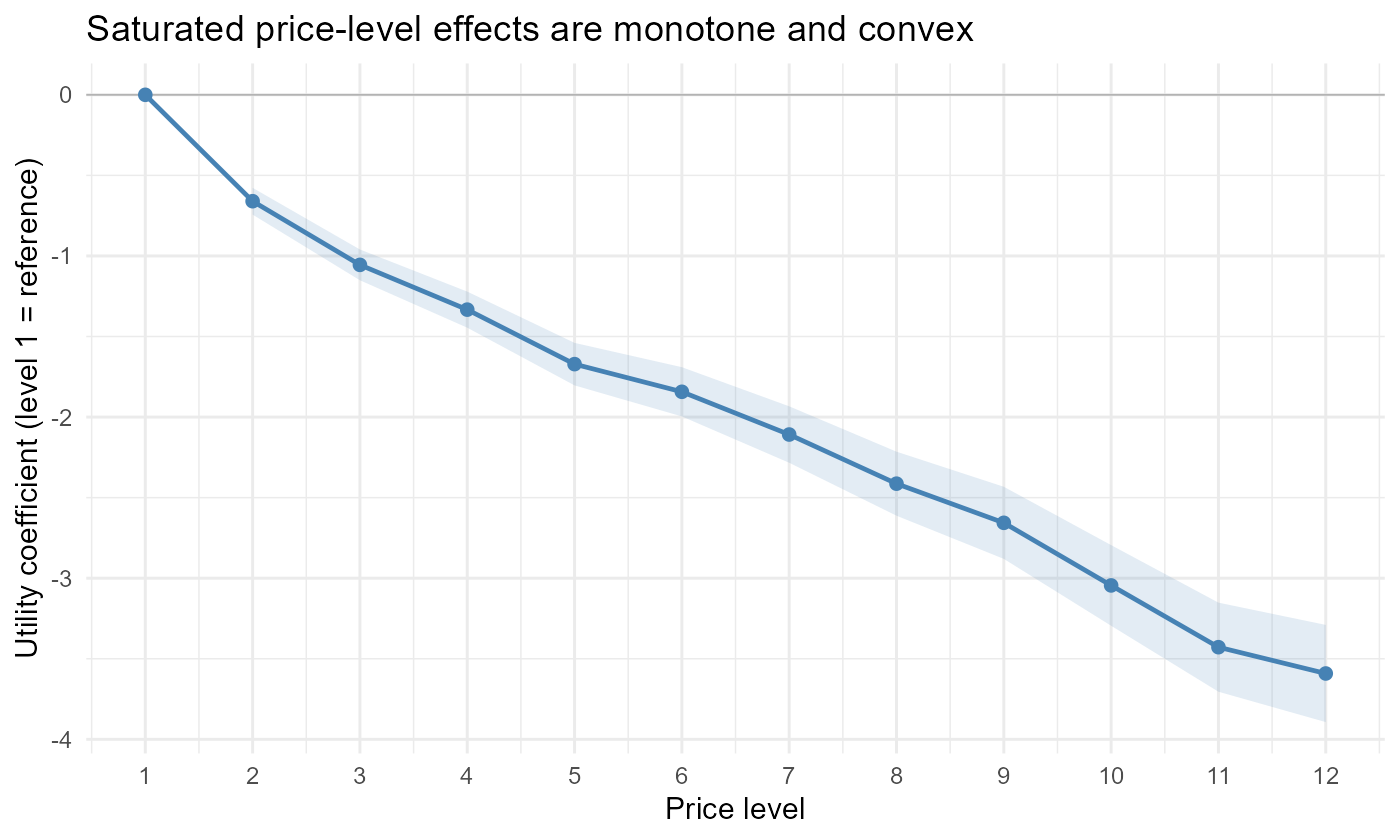
\includegraphics[width=0.6\linewidth,height=\textheight,keepaspectratio]{tae3.png}
\end{center}

Choice-set context added complementary signal. \texttt{is\_cheapest} and
\texttt{is\_dearest} encode price rank, while \texttt{price\_gap\_min}
and \texttt{price\_gap\_max} encode the magnitude of the differences.
Adding the price factor and rank terms improved CV from 1.15671 to
1.15160; the two gap terms then improved it to 1.147021. The gap
improvement was about 0.0046, several paired-bootstrap standard
deviations, and was achieved with only two additional parameters.

\subsection{Diverse xgboost component}\label{diverse-xgboost-component}

The second component is a wide-format \texttt{multi:softprob} xgboost
model with 73 boosting rounds (Chen and Guestrin 2016). It is weaker
alone (\textbf{1.178668 CV}) because it must learn the within-task
choice structure from raw columns, but its errors differ from the
conditional logit's. Out-of-fold weight search assigns it 20\% and
reduces CV log loss by 0.001927. The gain is small but directionally
stable: the ensemble beat m8trpg in 96.6\% of paired respondent
bootstrap samples.

\begin{center}
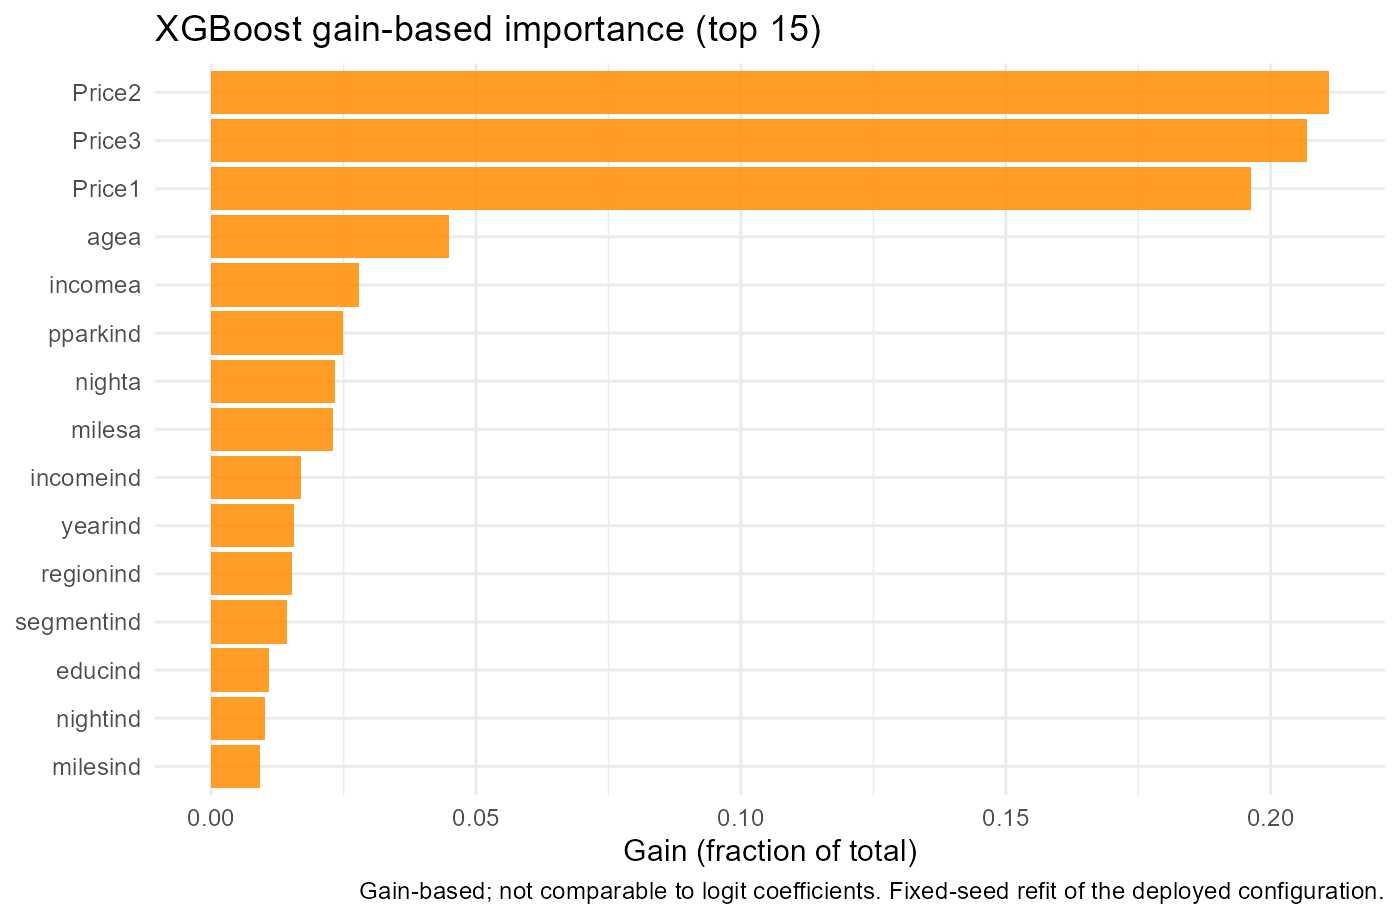
\includegraphics[width=0.6\linewidth,height=\textheight,keepaspectratio]{tae4.png}
\end{center}

\subsection{Neural ensemble diversity}\label{neural-ensemble-diversity}

Every flexible learner tried up to this point--CART, LASSO multinomial
regression, and multiple xgboost variants--remained tree-based and never
beat the structured logit alone. A small single-hidden-layer
feed-forward network (eight hidden units, weight decay 0.1, base R's
\texttt{nnet} (Venables and Ripley 2002)), trained on the same
wide-format attribute/price/covariate representation, scores
\textbf{1.190543 CV alone}--worse than either existing component--yet
contributes a genuinely different error pattern: fold-cross-fitted blend
weight 13--17\%, and a respondent-bootstrap 95\% interval for its
ensemble contribution of \textbf{{[}+0.000092, +0.002513{]}}, excluding
zero at our pre-stated ordinary significance threshold (though not under
a stricter correction for the architecture search that selected it). It
was the only candidate, out of several dozen tested after ensemble\_v11
(deeper networks, gradient-boosting variants with native categorical
handling, distribution-shift corrections, higher-order interactions, and
design-structure corrections described below), to clear this bar, and it
was submitted for exactly that reason.

\subsection{Set-context network}\label{set-context-network}

The final component learns, rather than hand-builds, choice-set context.
Every model above encodes each alternative's own attributes and price
plus a handful of hand-designed context features (\texttt{is\_cheapest},
\texttt{price\_gap\_min/max}). A feed-forward network instead takes, for
each alternative, its own features together with a permutation-invariant
summary of the \emph{other} alternatives in the same task (Zaheer et al.
2017)--in the spirit of set-pooling architectures for inputs with no
natural ordering. Scoring \textbf{1.261810 CV alone}, it is the weakest
standalone component yet contributes real, confirmed ensemble value via
the same weak-alone-but-diverse pattern already established for xgboost
and the shallow network. Its canonical five-fold CV gain was a wide,
low-confidence near miss (mean \textbf{+0.000153}, 64\% bootstrap win
rate), triggering our pre-registered escalation to six independent
fold-seed assignments; the pooled repeated-CV gain came back
\textbf{larger}, not smaller (\textbf{+0.001164}, 95\% interval
\textbf{{[}+0.000011, +0.002318{]}}, excluding zero, with all six
repeats positive). Before submission, the full-data build was required
to reproduce identically across two independent training runs (maximum
difference \textbf{0.0}), guarding against any silent nondeterminism in
the network fit.

Table 1 reports the main progression on comparable respondent-grouped
validation. Single-split figures are shown only for early models that
predated the canonical five-fold harness.

\begin{longtable}[]{@{}
  >{\raggedright\arraybackslash}p{(\linewidth - 6\tabcolsep) * \real{0.1800}}
  >{\raggedright\arraybackslash}p{(\linewidth - 6\tabcolsep) * \real{0.4600}}
  >{\raggedleft\arraybackslash}p{(\linewidth - 6\tabcolsep) * \real{0.2000}}
  >{\raggedleft\arraybackslash}p{(\linewidth - 6\tabcolsep) * \real{0.1600}}@{}}
\caption{Main model progression. Lower log loss is
better.}\label{tbl-models}\tabularnewline
\toprule\noalign{}
\begin{minipage}[b]{\linewidth}\raggedright
Model
\end{minipage} & \begin{minipage}[b]{\linewidth}\raggedright
Main change
\end{minipage} & \begin{minipage}[b]{\linewidth}\raggedleft
Local log loss
\end{minipage} & \begin{minipage}[b]{\linewidth}\raggedleft
Public
\end{minipage} \\
\midrule\noalign{}
\endfirsthead
\toprule\noalign{}
\begin{minipage}[b]{\linewidth}\raggedright
Model
\end{minipage} & \begin{minipage}[b]{\linewidth}\raggedright
Main change
\end{minipage} & \begin{minipage}[b]{\linewidth}\raggedleft
Local log loss
\end{minipage} & \begin{minipage}[b]{\linewidth}\raggedleft
Public
\end{minipage} \\
\midrule\noalign{}
\endhead
\bottomrule\noalign{}
\endlastfoot
Uniform benchmark & 0.25 per alternative & 1.3863 & 1.386 \\
mod1 & Linear conditional logit + ASCs & 1.2357 (holdout) & 1.270 \\
mod2b & Factor-coded attributes; identified alt dummies & 1.2186
(holdout) & -- \\
mod6 / mod7 & Price heterogeneity, then inside-good heterogeneity &
1.2049 / 1.2024 (holdout) & -- / 1.230 \\
mod8 & Segment-specific price and inside effects & 1.1665 (CV) & -- \\
m8tr & Task fatigue, region, parking & 1.1567 (CV) & -- \\
ensemble\_v9 & 70\% m8tr + 30\% xgboost & 1.1517 (CV) & 1.204 \\
m8trp & Saturated price + cheapest/dearest rank & 1.1516 (CV) & -- \\
m8trpg & Add price-gap magnitudes & 1.1470 (CV) & 1.213 \\
ensemble\_v11 & 80\% m8trpg + 20\% xgboost & 1.1451 (CV) & 1.202 \\
ensemble\_v11+MLP & +15\% feed-forward net & 1.1438 (CV) & 1.201 \\
+ set-context network & +11\% set-pooling net & 1.1435 (CV) & 1.200 \\
\textbf{+ segment-shift pruning (final)} & \textbf{Drop 2 unreliable
segment terms} & \textbf{1.1433 (CV)} & \textbf{1.200 / 1.199
private} \\
\end{longtable}

The experiments also established useful negative results:

\begin{itemize}
\tightlist
\item
  \textbf{Alternative choice structures.} Nested logit did not improve
  the bundle-versus-opt-out split. Full and price-only mixed logits
  improved training fit but not prediction for unseen respondents. Two
  observed-membership latent-class extensions (McLachlan and Peel 2000)
  were also null. A task-fatigue mixture scored 1.147826 CV and its
  class effects changed sign across folds. A more central model applied
  a class-specific multiplicative scale to every price-related utility
  term. It found stable classes at about 0.5 and 1.85--2.0 times normal
  price sensitivity across all folds, but scored 1.147629 versus
  1.147021 for m8trpg--a 0.0006 difference inside the noise floor. The
  discrete heterogeneity was real but redundant with continuous income,
  segment, and age interactions.
\item
  \textbf{Flexible learners.} CART, LASSO multinomial regression, and
  xgboost alone remained behind the structured logit. A long-format
  binary xgboost followed by within-task renormalization scored 1.2053
  versus 1.2042 for its wide multiclass counterpart; renormalization is
  not a genuine ranking objective. A subsequent \texttt{rank:ndcg} model
  grouped alternatives by choice task and improved xgboost's CV loss
  from 1.178668 to 1.163610, confirming that a true ranking loss learns
  useful within-task comparisons. A broader hyperparameter retune
  reached only 1.176029, however, and neither variant displaced
  ensemble\_v11. A teammate's random forest reported 1.1616 under a
  row-level split but 1.259 publicly, illustrating the leakage caused by
  splitting repeated tasks rather than respondents.
\item
  \textbf{Extra heterogeneity.} Attribute-by-segment terms, K-means
  personas, relative feature load, and additional price interactions
  with gender, urbanicity, or education did not generalize. Categorical
  price interactions with sparse night-driving and mileage bins caused
  quasi-separation; only balanced age bins gave a negligible gain.
  Extending cheapest/dearest rank flags to the other attributes was null
  because most level codes are unordered categories. Continuous
  three-way terms avoided the sparse-bin problem: Price \(\times\)
  income \(\times\) mileage had a negative coefficient in all five
  folds, but its ensemble gain was only 0.000495 and its
  respondent-bootstrap 95\% interval \textbf{{[}-0.000689, 0.001660{]}}
  crossed zero. Segment-specific mileage-price slopes were significantly
  harmful. A log-income transformation was also null.
\item
  \textbf{Combination methods.} A nested-CV conditional-logit stack on
  the base models' log probabilities (Wolpert 1992) scored 1.146126,
  marginally worse than the simple probability blend. With only two base
  models and a small minority weight on xgboost, the extra combiner
  flexibility added little. This conclusion held even after adding four
  more diverse components (below): a nested ridge-regularized log-linear
  opinion pool and a shallow xgboost meta-model both failed to beat
  simple arithmetic weighting a second time.
\end{itemize}

After ensemble\_v11, a further, larger round of experiments pursued
public leaderboard leaders' scores (reported near 1.186--1.190, against
our 1.202). None closed that gap, but several are worth recording as a
well-verified negative result rather than an unexamined ceiling:

\begin{itemize}
\tightlist
\item
  \textbf{Genuine ranking and regularized objectives.} A ranking-loss
  xgboost (\texttt{rank:ndcg} with task-level grouping), a re-tuned wide
  xgboost, and a regularized conditional logit fit via the
  stratified-Cox equivalence each modestly improved their own component
  (CV 1.1636, 1.1760, and 1.1643 respectively) and received stable
  minority weight in a combined blend, but an eight-component arithmetic
  blend of every model tried--including the neural network--reached only
  1.142112 CV. Its bootstrap interval barely cleared zero on the
  canonical split but, when re-tested with five additional independent
  fold assignments (repeated cross-validation, chosen specifically to
  distinguish a real gain from a favorable split), the pooled interval
  fell back across zero--a fold-assignment artifact, not a genuine
  improvement.
\item
  \textbf{Isolating and closing the two remaining threads.} The closest
  unconfirmed lead, a prior-smoothed price-reference feature bundled
  with a noisier attribute-familiarity term, was re-tested with the
  noisy term removed entirely (pre-registered, repeated cross-validation
  from the start): the isolated price-anchoring effect is real and
  directionally stable (its sign was negative in all 30 independent fold
  fits) but its size (about 0.0006) still sits inside the
  respondent-level noise floor. Separately, a weight-shared neural
  network trained on the exact four-way choice likelihood--the one
  untested combination of an exchangeable-alternative constraint with a
  flexible function class--screened positively but its canonical-CV gain
  shrank eight-fold versus the screen and its interval crossed zero
  comfortably. Two different function classes (tree and neural) now
  agree that the exact choice-likelihood objective was never the missing
  lever; the hand-built interaction structure is what does the real
  work.
\item
  \textbf{Distribution-shift correction by retraining, not just
  reweighted evaluation.} A genuine weighted-likelihood refit toward
  test-like respondents (density-ratio weights, following Shimodaira
  (2000)) was decisively harmful (bootstrap interval excluding zero on
  the harmful side): down-weighting training respondents costs more
  effective sample size than it gains from targeting the shifted
  population.
\item
  \textbf{Exact conditional-logit-consistent gradient boosting.} Wide
  multiclass and ranking-loss xgboost do not directly optimize the
  four-way softmax likelihood the way \texttt{mlogit} does. A custom
  xgboost objective enforcing the true multinomial gradient (verified
  against finite differences) failed cold-start, confirming that
  m8trpg's hand-built interaction structure, not the loss function, was
  doing the real work; used as a small residual correction on top of
  m8trpg's own fitted utility it gave a tiny, statistically unconfirmed
  gain.
\item
  \textbf{A confirmed design-rotation structure.} Fingerprinting each
  respondent's complete ordered 19-task design sequence shows the survey
  reuses a pool of only \textbf{299 distinct questionnaire versions}
  across train and test combined, consistent with standard commercial
  CBC rotation defaults--a stronger, previously undetected version of
  the 98.5\% single-task recurrence above. A cross-fitted, utility-space
  penalized correction to the opt-out option keyed by version was tested
  but rejected: each version has only 3--5 sharing respondents, too few
  to support even one well-shrunk parameter without being dominated by a
  single respondent.
\item
  \textbf{Two more tree-learner families and a pre-registered
  architecture search.} LightGBM (Ke et al. 2017) and CatBoost
  (Prokhorenkova et al. 2018), whose native categorical-splitting
  mechanisms differ from xgboost's, both received zero ensemble weight.
  A 24-configuration neural architecture search, with its multiplicity
  correction fixed \emph{before} seeing any results, found a modestly
  better network but correctly rejected it under the pre-declared rule.
\item
  \textbf{A further wave of four independently-verified experiments.}
  Learned choice-set-crowding features and a stagewise, component-wise
  boosting correction on m8trpg's fitted utility were both
  consistently-signed but tiny near misses that failed repeated
  cross-validation (gains of +0.000102 and +0.000038); a
  curvature-shrunk version of the saturated price factor was a clean,
  decisive reject (-0.0019), confirming that factor is not overfit; a
  calibrated radial-basis-function support vector machine--a materially
  different function class from every tree or neural component
  tried--scored worse alone than any other component and, unlike xgboost
  or the shallow network, made the ensemble worse rather than better.
\end{itemize}

These results show why selection used predictive loss rather than
p-values: several added terms had very small p-values yet worsened the
holdout score.

\section{Public versus private leaderboard
fit}\label{public-versus-private-leaderboard-fit}

The public leaderboard evaluates approximately 70\% of the 4,997 test
tasks; the remaining 30\% formed the private leaderboard, unseen until
the competition closed. The public gap has not been constant: mod1 was
0.034 worse than local validation, mod7 0.028 worse, ensemble\_v9 0.052
worse, and ensemble\_v11 0.057 worse. This prevented us from projecting
the private score by simply adding a fixed correction to CV.

Now that the private leaderboard is visible, we can check this directly
rather than only simulate it. Across 18 team submissions with both
scores recorded, public and private log loss correlate at
\textbf{r=0.979}; private was on average 0.004 \emph{better} than public
(sd 0.005, max difference 0.013)--the public leaderboard was, in
practice, an unbiased, low-noise proxy for private here. CV predicted
private slightly less tightly than public (r=0.787 vs.~0.845; mean gap
0.052 vs.~0.057), consistent with private being a smaller, noisier
panel, as our bootstrap simulation anticipated. Ranking our own
progression by private score alone does not perfectly reproduce the CV
ranking--ensemble\_v9 (1.152 CV, weakest of the group) edges out both
set-context and segment-shift pruning (1.199 private each) at 1.197--but
the spread across seven models is only 0.018, well inside the
paired-noise band this report already quantifies: confirmation of, not
an exception to, our own thesis that small private-rank differences here
reflect noise, not quality.

\subsection{Team submissions}\label{team-submissions}

For completeness, every teammate's independently submitted model is
listed below, code-reviewed for validation soundness, not only the
zhenhao-branch progression of Section 2.

\begin{longtable}[]{@{}
  >{\raggedright\arraybackslash}p{(\linewidth - 8\tabcolsep) * \real{0.3800}}
  >{\raggedright\arraybackslash}p{(\linewidth - 8\tabcolsep) * \real{0.1000}}
  >{\raggedright\arraybackslash}p{(\linewidth - 8\tabcolsep) * \real{0.1200}}
  >{\raggedright\arraybackslash}p{(\linewidth - 8\tabcolsep) * \real{0.1200}}
  >{\raggedright\arraybackslash}p{(\linewidth - 8\tabcolsep) * \real{0.2800}}@{}}
\caption{Benchmark comparison.}\tabularnewline
\toprule\noalign{}
\begin{minipage}[b]{\linewidth}\raggedright
Model
\end{minipage} & \begin{minipage}[b]{\linewidth}\raggedright
CV
\end{minipage} & \begin{minipage}[b]{\linewidth}\raggedright
Public
\end{minipage} & \begin{minipage}[b]{\linewidth}\raggedright
Private
\end{minipage} & \begin{minipage}[b]{\linewidth}\raggedright
Validation
\end{minipage} \\
\midrule\noalign{}
\endfirsthead
\toprule\noalign{}
\begin{minipage}[b]{\linewidth}\raggedright
Model
\end{minipage} & \begin{minipage}[b]{\linewidth}\raggedright
CV
\end{minipage} & \begin{minipage}[b]{\linewidth}\raggedright
Public
\end{minipage} & \begin{minipage}[b]{\linewidth}\raggedright
Private
\end{minipage} & \begin{minipage}[b]{\linewidth}\raggedright
Validation
\end{minipage} \\
\midrule\noalign{}
\endhead
\bottomrule\noalign{}
\endlastfoot
Zeening: RF, grid-searched (\texttt{rf\_gridsearch}) & 1.162 & 1.259 &
1.253 & row-level split--\textbf{leaky} \\
Zeening: RF+XGB+glmnet blend (\texttt{019\_blended.R}) & -- & 1.216 &
1.226 & respondent-grouped--sound \\
Imelda: 3-way MNL ensemble & 1.228 & 1.263 & 1.254 &
respondent-grouped--sound \\
Imelda: MNL + xgboost & 1.186 & 1.255 & 1.247 &
respondent-grouped--sound \\
Imelda: MNL + covariate interactions & -- & 1.249 & 1.245 &
respondent-grouped--sound \\
Imelda: as above, blended toward uniform & 1.203 & 1.245 & 1.241 &
respondent-grouped--sound \\
Clarence: xgboost (task-based split) & -- & 1.221 & 1.216 & task-based
split--\textbf{leaky} \\
Clarence: ensemble, honest re-weighting & 1.165 & 1.224 & 1.219 &
respondent-grouped--sound (our fix) \\
\end{longtable}

``--'' marks a CV never captured. Two submissions were leaky at build
time (Zeening's first: random row split; Clarence's: task-number split,
not respondent) and had no trustworthy internal CV as a result; both
were later fixed--we rebuilt Clarence's ensemble with honest
fold-cross-fitted weights, and Zeening independently corrected her own
methodology, which we verified implements respondent-grouped CV
throughout. Every properly-validated teammate submission (five of eight)
landed in a tight 1.19--1.26 band on both leaderboards with
mlogit-family-sized gaps, reinforcing that respondent-grouped
validation, not model family or author, is what separates a trustworthy
estimate from a misleading one here. One further submission,
\texttt{hierarchical\_pool\_v18\_balanced} (public 1.200, private
\textbf{1.194}, better than every model above), could not be traced to
any script despite an exhaustive git-history search and is reported
without further interpretation.

\subsection{Distribution shift and experimental
blocks}\label{distribution-shift-and-experimental-blocks}

Adversarial validation using respondent covariates distinguished train
from test at \textbf{AUC 0.634}, confirming covariate shift. Income was
the dominant separator: median income was 60,000 in train and 80,000 in
test, and some top brackets were more than three times as prevalent in
test. However, this did not justify an unvalidated correction.
Test-likeness weighting raised m8trpg's OOF loss from 1.1470 to about
1.1577, but the highest-income training tercile actually had the best
loss. Two income-reweighting estimates put the shift's contribution to
the 0.057 CV-public gap near 0.010 (about 18\%), yet a
respondent-bootstrap 95\% interval of \textbf{{[}-0.0057, 0.029{]}}
includes zero. We also tested a genuine density-ratio weighted refit,
with both fitting and held-out evaluation targeted toward test-like
respondents (Shimodaira 2000). Even the gentlest weight was harmful in
every fold: target-weighted loss rose from 1.159787 to 1.161203, and the
95\% interval for its gain was \textbf{{[}-0.002614, -0.000422{]}}.
Reweighting reduced effective sample size enough that variance
outweighed any targeting benefit. Log-income interactions did not
improve validation. We therefore treat income shift as a real risk
factor, not as a quantified causal explanation or a validated
correction.

A second, more extreme shift was found by directly auditing the model's
existing parameters rather than proposing a new one. The market-segment
covariate shifts far more sharply than income: segment 6 is 27.0\% of
the 1,135 training respondents but 0\% of the 263 test respondents,
while segments 3 and 5 are only 9.4\% of training combined but 68.8\% of
test--an adversarial-validation classifier on segment alone reaches
\textbf{AUC 0.898}, dwarfing income's 0.634. A full-data coefficient
audit of \texttt{m8trpg} found that segments 3 and 5's opt-out-margin
deviation terms are statistically indistinguishable from zero even on
the full training set (p=0.758, p=0.404) while their price-sensitivity
counterparts are highly significant (p\textless1e-10)--two already-weak,
already-deployed parameters whose loss-function weight explodes roughly
sevenfold between training and test. Dropping only these two terms
improved respondent-grouped CV on the whole population (not merely a
subgroup), amplified monotonically on the 30\% of training respondents
most similar to test, and survived repeated CV at the full-ensemble
level (Section 2)--the only case here where auditing an already-deployed
parameter against a known shift, not a new mechanism, produced a
promotable improvement.

The conjoint experiment is also heavily blocked: each task position
draws from about 296 exact designs, seen by 3.8 respondents on average,
and \textbf{98.5\%} (4,921/4,997) of test tasks exactly repeat a train
design. Cross-fitted empirical choice-share shrinkage improved 1.145094
only to 1.144742, within the paired noise floor; stronger use of cell
frequencies hurt because three or four observations cannot estimate a
reliable four-way share. The overlap is reassuring for design support
but does not remove respondent-composition risk.

\subsection{Why the ensemble should be
retained}\label{why-the-ensemble-should-be-retained}

We directly tested whether xgboost caused a complexity or overfitting
penalty by submitting m8trpg alone. Despite being simpler, it scored
\textbf{1.213 public}, a 0.065979 CV-public gap--the largest among our
trustworthy models--whereas ensemble\_v11 scored 1.202 with a 0.056906
gap. Removing the weaker learner made the public result worse, so the
20\% xgboost component is genuine variance reduction, not needless
complexity. Adding the neural-network component (Section 2.3) then
improved both CV (1.145094 to 1.143789) and public score (1.202 to
1.201) together--a 0.057211 gap, consistent with the established
0.052--0.057 pattern, and the first refinement whose public result was
checked against its CV-predicted direction and matched.

A second submission reinforces this. Combining the neural network with
an additional price-by-income-by-mileage interaction reached the best
pre-submission CV of any untested candidate at the time (1.143328), but
its bootstrap interval against the current best already crossed zero;
submitted anyway as the best available honest bet, it scored
\textbf{1.210 public}--worse than the retained model. Its CV-public gap
(0.0667) is the largest in the project, close to the plain-logit gap
rather than the ensemble-class pattern.

A third submission then broke the losing streak. The set-context network
(Section 2.4) cleared our bar via repeated cross-validation and was
added at an 11.1\% weight, frozen from the mean of six cross-fitted fold
weights and locked behind a full-data build required to reproduce
identically across two independent runs. It scored \textbf{1.200
public}, a 0.056467 CV-public gap--again inside the 0.052--0.057
ensemble-class pattern, and the second confirmed CV-predicted direction.

A fourth submission, segment-shift pruning, is smaller and more targeted
than any of the above--a full-ensemble CV improvement of only 0.000278,
an order of magnitude below the others. It scored \textbf{1.200 public},
identical to the prior submission at three-decimal precision--below both
Kaggle's rounding granularity and our 0.001 noise floor, so this result
is genuinely uninformative rather than confirmatory. We retain it on the
strength of its CV evidence (Section 2) and its structural rationale,
not because the public leaderboard confirmed it.

Leaderboard differences must also be read at the respondent level. A
snapshot of the real public leaderboard (43 teams, 27 July 2026) placed
us 16th of 43 at 1.201; the top 18 teams span only 0.016 of log loss,
and 34 of 43--including the leader--sit within one
noise-standard-deviation of our score. Resampling public-sized sets of
184 whole respondents from OOF predictions gave a single-score standard
deviation of \textbf{0.0225}, 2.14 times the naive row-level estimate,
and \textbf{64.6\%} of equally generated sample pairs differed by at
least 0.015--comparable to the gap separating most of the leaderboard's
middle tier. This compression is visible directly in
independently-scored results, not just our own simulation, and is
consistent with most nearby leaderboard gaps reflecting sampling noise
rather than a missing modeling breakthrough. Our best defense is
respondent-grouped CV, observed heterogeneity, and a diverse
ensemble--not tuning to one public split.

Finally, now that the leaderboard has closed: one untracked submission
scored better privately than our selected final (Section 3.1)--never a
candidate at selection time, and not read as proof of a better model
given the size of the gap relative to this section's own noise band. We
report it for completeness.

\section{Insights and limitations}\label{insights-and-limitations}

Several behavioral insights were especially robust, holding across
respondent-grouped validation rather than reflecting training-set fit
alone. Price is the dominant driver of choice and its effect is
nonlinear: a variable-importance screen entered Price ahead of every
safety attribute, and recoding the attribute levels as factors rather
than a single linear slope improved validation from 1.236 to roughly
1.219. The price levels themselves proved monotone and convex once
saturated (about -0.66 at level 2 falling to -3.64 at level 12), and
deliberately shrinking that curve toward a smoother shape made the model
decisively worse, so the curvature is real signal rather than
overfitting.

Observed respondent characteristics also transfer to new people while
respondent-specific tastes do not. A panel mixed logit with random
parameters on all attributes fit the training data far better than its
fixed counterpart (log-likelihood -16,449 versus -20,432) yet scored
worse on held-out validation (1.247 versus 1.236)--a textbook
overfitting result, since the test respondents (Cases 1,136 to 1,398)
are entirely new people with nothing for memorized tastes to transfer
to. Heterogeneity carried through observed covariate interactions drove
the project's single largest gain instead: price-by-covariate
interactions on income, age, mileage, and night driving improved
validation from 1.219 to 1.205, and segment interactions improved it
again.

Task position matters too, but through a sharper channel than generic
fatigue. The opt-out share rises from about 24\% at Task 1 to about 34\%
by Tasks 15 to 19, and interacting task position with both price and the
inside-good indicator leaves only the price interaction significant.

The final insight is structural rather than behavioral, and became the
final model. The market-segment mix shifts far more sharply between
train and test than any other covariate: segment 6 is 27.0\% of training
respondents but 0\% of test, while segments 3 and 5 rise from 9.4\% of
training combined to 68.8\% of test. A coefficient audit found that
these two segments' opt-out-margin terms were statistically
indistinguishable from zero even on the full training data, while their
price-sensitivity counterparts were highly significant. Dropping only
those two already-weak, already-deployed parameters improved
respondent-grouped validation across the whole population, and more so
on the training respondents most similar to test.

Limitations remain. Validation log loss is consistently optimistic and
the gap to the public leaderboard widens with model complexity: 0.034
for the simplest model, 0.028 at mid-size, but 0.052 to 0.057 for the
best ensembles. The model family also shows clear diminishing returns:
after the gains from observed heterogeneity and the price curve, a large
and diverse set of further extensions--alternative choice structures,
higher-order interactions, distribution-shift reweighting, bagging,
additional tree and neural learners, and learned stacking--each moved
cross-validation by less than the roughly 0.001 paired-comparison noise
floor, and none was promoted. The final model's 1.200 public and 1.199
private reflects that ceiling. Stated choices also carry irreducible
noise, since respondents are inconsistent across their own 19 tasks and
unobserved tastes escape the observed covariates.

\section{Further work}\label{further-work}

A few threads were flagged as promising but left unresolved by the
competition deadline. The \texttt{hierarchical\_pool\_v18\_balanced}
submission (Section 3.1) outperformed every traced model on the private
leaderboard; reconstructing its methodology, or re-deriving whatever
mechanism it captured, is the single highest-value open item. The
confirmed design-rotation structure (299 distinct questionnaire
versions, Section 3.2) was diagnosed but not exploited--a hierarchical,
more heavily shrunk version-level correction with informative priors
borrowed across similar versions might succeed where our under-powered
per-version attempt did not. More generally, the income and segment
shift analyses point toward reweighting schemes evaluated on a genuinely
test-like validation slice rather than the full training panel, which
our simple density-ratio refit did not have the sample size to support.
Finally, several near-miss features (learned choice-set-crowding,
stagewise boosting corrections on m8trpg's utility) sit just inside the
noise floor on current evidence; a larger repeated-CV budget, or pooling
across teams' independent implementations, could resolve whether they
are real but small effects or artifacts of a single fold assignment.

\section*{References}\label{references}
\addcontentsline{toc}{section}{References}

\protect\phantomsection\label{refs}
\begin{CSLReferences}{1}{1}
\bibitem[\citeproctext]{ref-chen2016}
Chen, Tianqi, and Carlos Guestrin. 2016. {``{XGBoost}: A Scalable Tree
Boosting System.''} \emph{Proceedings of the 22nd ACM SIGKDD
International Conference on Knowledge Discovery and Data Mining},
785--94. \url{https://doi.org/10.1145/2939672.2939785}.

\bibitem[\citeproctext]{ref-croissant2020}
Croissant, Yves. 2020. {``Estimation of Random Utility Models in {R}:
The {mlogit} Package.''} \emph{Journal of Statistical Software} 95 (11):
1--41. \url{https://doi.org/10.18637/jss.v095.i11}.

\bibitem[\citeproctext]{ref-ke2017}
Ke, Guolin, Qi Meng, Thomas Finley, et al. 2017. {``{LightGBM}: A Highly
Efficient Gradient Boosting Decision Tree.''} \emph{Advances in Neural
Information Processing Systems 30 (NeurIPS 2017)}.

\bibitem[\citeproctext]{ref-mclachlan2000}
McLachlan, Geoffrey J., and David Peel. 2000. \emph{Finite Mixture
Models}. Wiley. \url{https://doi.org/10.1002/0471721182}.

\bibitem[\citeproctext]{ref-prokhorenkova2018}
Prokhorenkova, Liudmila, Gleb Gusev, Aleksandr Vorobev, Anna Veronika
Dorogush, and Andrey Gulin. 2018. {``{CatBoost}: Unbiased Boosting with
Categorical Features.''} \emph{Advances in Neural Information Processing
Systems 31 (NeurIPS 2018)}.

\bibitem[\citeproctext]{ref-shimodaira2000}
Shimodaira, Hidetoshi. 2000. {``Improving Predictive Inference Under
Covariate Shift by Weighting the Log-Likelihood Function.''}
\emph{Journal of Statistical Planning and Inference} 90 (2): 227--44.
\url{https://doi.org/10.1016/S0378-3758(00)00115-4}.

\bibitem[\citeproctext]{ref-venables2002}
Venables, William N., and Brian D. Ripley. 2002. \emph{Modern Applied
Statistics with {S}}. Fourth. Springer.
\url{https://doi.org/10.1007/978-0-387-21706-2}.

\bibitem[\citeproctext]{ref-wolpert1992}
Wolpert, David H. 1992. {``Stacked Generalization.''} \emph{Neural
Networks} 5 (2): 241--59.
\url{https://doi.org/10.1016/S0893-6080(05)80023-1}.

\bibitem[\citeproctext]{ref-zaheer2017}
Zaheer, Manzil, Satwik Kottur, Siamak Ravanbakhsh, Barnabas Poczos,
Ruslan Salakhutdinov, and Alexander J. Smola. 2017. {``Deep Sets.''}
\emph{Advances in Neural Information Processing Systems 30 (NeurIPS
2017)}.

\end{CSLReferences}




\end{document}
